\section{Evaluation}
\label{ch:eval}

\epigraph{If a machine is expected to be infallible, it cannot also be intelligent.}{Alan Turing}

In this chapter, the author conduct evaluations of the collected data.
The data is collected from 21 subjects, and 189 clickstream data are collected in total. 
Each clickstream contains action-level data with a stay duration
of a specific page, for instance, the study also collected a URL as a step of clickstream 
if a participant uses back button rollback to a previously visited page
without requesting server. 
\emph{A clickstream also has a subjective difficulty score that measured from the questionnaire 
through a self-rating scale (shown in Appendix \ref{appendix:b}) after the completion of each task.}

\subsection{Subjective Task Difficulty}
\label{sec:task-diff}

This section discusses the subjective task difficulty qualitatively and quantitatively.
Figure \ref{fig:difficulty} illustrates a normalized (raw scores are listed in 
Appendix \ref{appendix:c} Table \ref{table:diff-raw}) subjective difficulty score 
with respect to all tasks.

\begin{figure}[H]
    \centering
    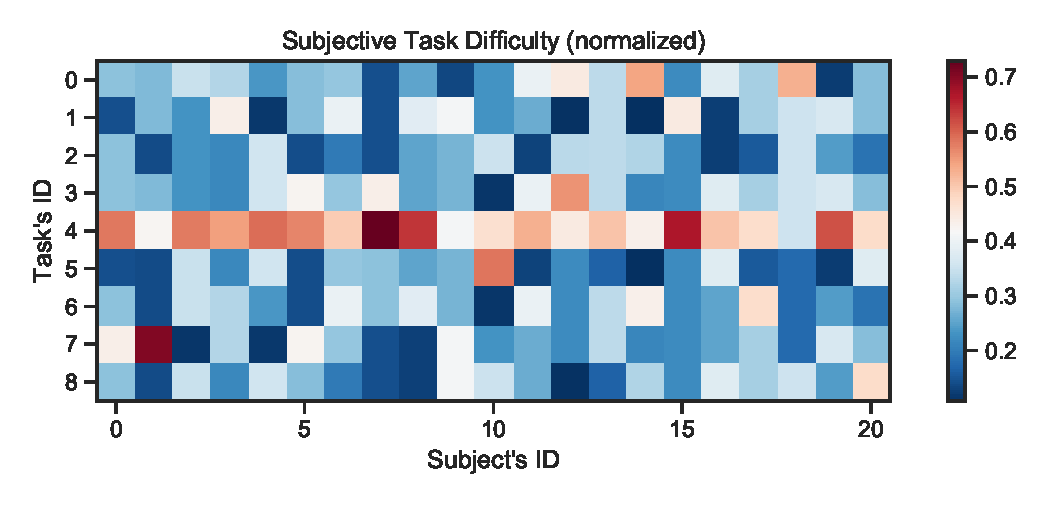
\includegraphics[width=0.7\textwidth]{figures/difficulty}
    \caption{Subjective difficulty score: each column indicates an individual subject 
    and each row indicates a browsing task. \emph{TasksID} from 0 to 8 represent 
    Amazon Goal Oriented Task, Amazon Fuzzy Task, Amazon Exploring Task; 
    Medium Goal Oriented Task, Medium Fuzzy Task, Medium Exploring Task, 
    Dribbble Goal Oriented Task, Dribbble Fuzzy Task, 
    and Dribbble Exploring Task respectively.
    From this heat map, one can observe Medium Fuzzy Task is the most challenging task 
    according to the subjects voted subjective difficulty, 
    a Mann-Whitney U significant test justifies this observation.}
    \label{fig:difficulty}
\end{figure}

The purpose of measuring task difficulty is to give a verification of task design,
and understanding how subjects votes the difficulty in different browsing behaviors.
Therefore, a significant test is considered with the null hypothesis ($H_0$): 
the difficulty of fuzzy task is not significantly greater than exploring task 
and alternative hypothesis ($H_1$): 
the difficulty of fuzzy task is significantly greater than exploring task. 

A non-parametric one-tailed Mann-Whitney U test \cite{mann1947test} is conducted as follows. 
Under the null hypothesis, $p=2.54\times 10^{-5} < 0.05$, reject $H_0$.
Similarly, one can compare difficulty score on goal oriented task and exploring task (with corresponding hypothesis, 
$p=0.00534 < 0.05$), difficulty score on fuzzy task and goal oriented task (with corresponding hypothesis, 
$p=0.0145 < 0.05$), all rejects $H_0$. Therefore one can conclude that the task difficulty is ordered
as follows: \emph{difficulty of fuzzy task $>$ difficulty of goal oriented task $>$ difficulty of exploring task},
which means exploring tasks have lower effort in clickstream, and effort of doing fuzzy task gains highest effort.

\subsection{Browsing Behavior Classification}

As discussed in Section \ref{sec:task-design}, three types of browsing behavior are described. 
In this section, the author of the thesis provides two types of evaluations to 
interpret the browsing behavior classification.

First, the thesis evaluates the indication of general features browsing behavior:
task efficiency (Section \ref{sec:efficiency}), 
number of actions in an action path 
as well as the total stay duration in the action path.
Then APM is implemented by using the action-level clickstream data and stay duration of each page,
which was described in Section \ref{sec:recurrent-unit} and \ref{sec:mark-interpretation}.

\subsubsection{Interpretation based on General Features}
\label{sec:inter-general-feature}

\textbf{As a baseline and a comparison to the APM for the classification performance}, 
the \emph{completion efficiency}, 
\emph{total time duration of a task} 
as well as \emph{total number of actions of a task} are used for
browsing behavior classification in support vector machine (SVM) \cite{suykens1999least}.

\emph{Note that the shortest path of entire clickstream defines the completion efficiency,
 moreover, the completion efficiency can only be determined if and only if the clickstream
 is given, in a sense, it carries latent information of browsing behavior.}

SVM with the polynomial kernel is applied with gird-search.
The best classification precision is 0.53 (with $C=4.5$ and $\gamma = 1.5$, 
which are the searched hyper-parameters in SVM model).
The micro average F1 score is also 0.53, which is better than random (0.33).
The t-SNE visualization is showed with pairs of features for graphical insights
in Figure \ref{fig:general-amazon}.

\begin{figure}
    \centering

    \begin{subfigure}[b]{0.45\textwidth}
        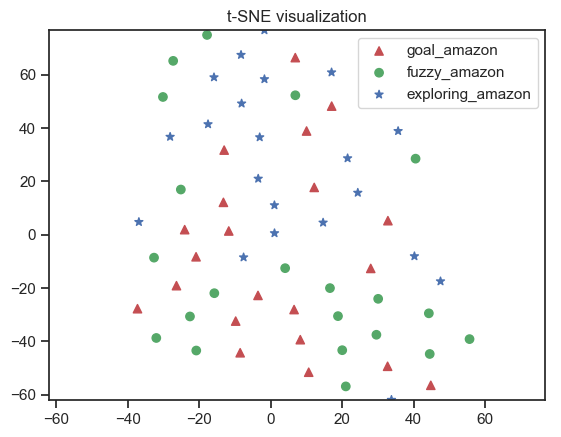
\includegraphics[width=1\textwidth]{figures/tsne-amazon}
        \caption{}
        \label{fig:tsne-amazon}
    \end{subfigure}
    \begin{subfigure}[b]{0.45\textwidth}
        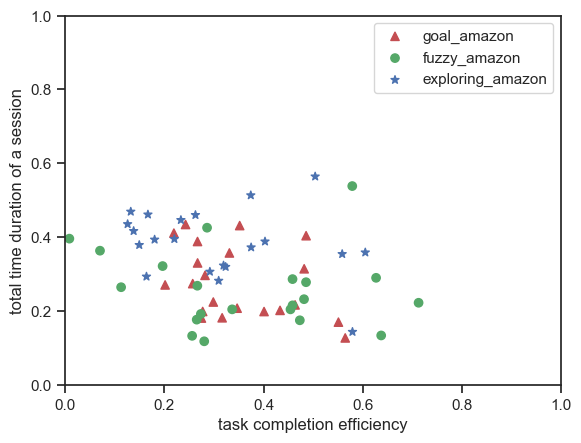
\includegraphics[width=1\textwidth]{figures/2d-eff-dur-amazon}
        \caption{}
        \label{fig:2d-eff-dur-amazon}
    \end{subfigure}
    \begin{subfigure}[b]{0.45\textwidth}
        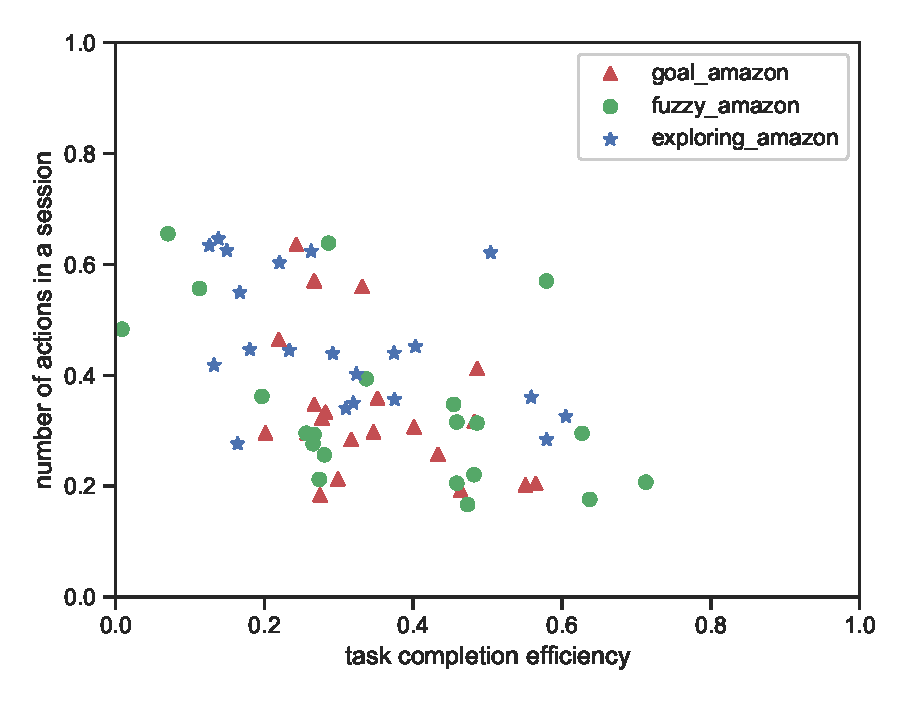
\includegraphics[width=1\textwidth]{figures/2d-eff-len-amazon}
        \caption{}
        \label{fig:2d-eff-len-amazon}
    \end{subfigure}
    \begin{subfigure}[b]{0.45\textwidth}
        \includegraphics[width=1\textwidth]{figures/2d-len-dur-amazon}
        \caption{}
        \label{fig:2d-len-dur-amazon}
    \end{subfigure}

    \caption{In these figures, \ref{fig:tsne-amazon} shows the t-SNE projection
    of completion efficiency, total time duration and number of actions for three different behavior;
    \ref{fig:2d-eff-dur-amazon} is a 2D comparison of using completion efficiency and total time duration;
    \ref{fig:2d-eff-len-amazon} provides a 2D comparison of using completion efficiency and number of actions;
    \ref{fig:2d-len-dur-amazon} shows a 2D comparison of using number of actions and total time duration.
    From t-SNE visualization, one can observe that exploring tasks tend to centralized on the right and goal-oriented
    tasks and fuzzy tasks tend to centralized on the left, which indicates that exploring behaviors tend to classifiable
    comparing to the other two behaviors. According to the rest of feature comparison visualizations, the completion efficiency and total time duration
    contributes more to interpret exploring behavior, and the number of actions tent to
    contributes more to interpret goal-oriented task.}
    \label{fig:general-amazon}
\end{figure}

To better understand the meaning of classification, a randomized decision tree is also applied
(ExtraTreesClassifier in \emph{scikit-learn} \cite{scikit-learn}
with default parameter settings)
that gives the importance of the used features: \textbf{\emph{total time duration and number of actions
of a task are more important than self-defined completion efficiency.}}

Moreover, one-tailed Mann-Whitney U test is used in each pair of these features.
For instance, the null hypothesis ($H_0$): the completion efficiency of the goal-oriented task 
is not significantly greater than exploring task. The result shows $p = 0.0019 < 0.05$ reject $H_0$, 
which means the completion efficiency of goal-oriented task 
is significant efficient than than exploring task.

Similarly, one can conduct the significant test with similar hypothesis 
to all comparable combinations 
as listed in Table \ref{table:sig-test-efficiency}, \ref{table:sig-test-duration}, and \ref{table:sig-test-actions}.

\begin{table}[H]
    \small
    \centering
    \caption{One-tailed significant tests for completion efficiency in different browsing behaviors.
    The null hypothesis in this table, for instance, completion efficiency of the fuzzy task
    is \emph{not} significant efficient than the goal-oriented task, the result $p=0.45>0.05$ which means
    accept $H0$. Similar to others.}
        \begin{tabular}{cccc}
            \toprule
              v.s.             & efficiency goal & efficiency fuzzy & efficiency explore \\
            efficiency goal    & N/A             & reject           & reject             \\
            efficiency fuzzy   & accept          & N/A              & reject             \\
            efficiency explore & accept          & accept           & N/A                \\
            \bottomrule
        \end{tabular}
        \label{table:sig-test-efficiency}
\end{table}

\begin{table}[H]
    \small
    \centering
    \caption{One-tailed significant tests for total stay duration of a task in different browsing behaviors.
    The null hypothesis in this table, for instance, total stay duration of the fuzzy task
    is \emph{not} significant stay longer than goal-oriented task, the result $p=0.41>0.05$ which means
    accept $H0$. Similar to others.}
        \begin{tabular}{cccc}
            \toprule
              v.s.             & duration goal & duration fuzzy & duration explore \\
            duration goal      & N/A & reject & reject \\
            duration fuzzy     & accept & N/A & reject \\
            duration explore   & accept & accept & N/A \\
            \bottomrule
        \end{tabular}
        \label{table:sig-test-duration}
\end{table}

\begin{table}[H]
    \small
    \centering
    \caption{One-tailed significant tests for total number of actions of a task in different browsing behaviors.
    The null hypothesis in this table, for instance, total number of actions of the fuzzy task
    is \emph{not} significant performs more actions than the goal-oriented task, the result $p=0.019<0.05$ which means
    reject $H0$. Similar to others.}
        \begin{tabular}{cccc}
            \toprule
              v.s.             & actions goal & actions fuzzy & actions explore \\
              actions goal      & N/A & accept & reject \\
              actions fuzzy     & reject & N/A & accept \\
              actions explore   & accept & reject & N/A \\
            \bottomrule
        \end{tabular}
        \label{table:sig-test-actions}
\end{table}

As a summary, the insights of each feature are concluded as follows:

\begin{itemize}
    \item \textbf{Completion efficiency}: the completion efficiency of goal-oriented and fuzzy behavior is significant efficient than exploring behavior;
    \item \textbf{Number of actions}: the number of actions of goal-oriented behavior is significantly lower than fuzzy and exploring behaviors.
    \item \textbf{Total stay duration}: the total stay duration of exploring behavior is significantly higher than goal-oriented and fuzzy behaviors.
\end{itemize}

Furthermore, the completion efficiency and total stay duration are more critical than others for indication of exploring behavior,
also, the number of actions are more important than others for indication of goal-oriented behavior.

\subsubsection{Interpretation based on Action Path}
\label{sec:inter-action-path}

To use the full capacity of action path data and learn the deep inside structures of an action path,
this section uses the entire clickstream and its corresponding
action-level stay duration as input, three ending mark (<EOA\_GOAL>, <EOA\_FUZZY>, and <EOA\_EXPLORE>) 
as classification outputs. Then a single GRU-like layer based APM is presented for
the classification of the three types of browsing behaviors.

The tunable training parameters are equivalent to standard GRU: 
The latent dimension is 10, the training process feeds 132 clickstreams as training data,
38 clickstreams as validation, then propagate 500 epochs with a batch size of 32. 
In the training process, Adam optimizer is used,
 categorical cross-entropy loss as well as L2 regularizer (with 0.0000001) with early stopping (patient 1000),
the total number of trainable parameters is 90323.

At the end of training, 19 clickstreams as the testing dataset are evaluated. 
\textbf{The APM archived precision of 1.00\%} of browsing behaviors classification, i.e., 100\% of accurate.
Note that the training set is randomly selected from all participants, which is supervised
with k-Fold cross validation \cite{kohavi1995study} while training, the reason for
using k-Fold other than else is discussed in Section \ref{sec:decision}.

\begin{figure}[H]
    \centering
    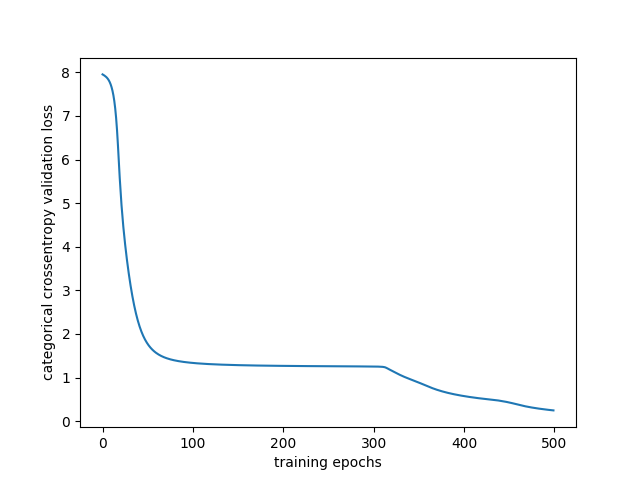
\includegraphics[width=0.55\textwidth]{figures/class-loss}
    \caption{Categorical cross-entropy validation loss curve while 500 epochs. 
    The curves indicates the training process is not an overfitting since the loss is not increasing but keep reducing.}
    \label{fig:class-loss}
\end{figure}

One can observe that the training process is not an overfit, and the validation loss is 
still not increase after 500 epochs. Thus, a single GRU-like layer in APM 
remains a large expressive generalization performance 
(100\% accurate for three browsing behavior classification). Therefore
the author expect to collect more data to verify whether the APM applicable to a large dataset.

In addition, the APM feeds the entire clickstream and time duration as inputs, 
therefore the entire clickstream contains pieces of information regarding the number of actions
as well as completion efficiency and more latent pieces of information. 
Consequently, one can conclude that the APM works
\emph{perfectly on the classification of three different browsing behavior}. 
Since the experiment is only designed for three types of behavior, and the learning curve
shows the APM still has the capacity and generalization ability to 
classify more precise categories of browsing behavior, a future investigation on
more categories may be worthwhile.

\subsection{Optimal Action Path Context}
\label{sec:eval-optimal}

This section evaluates the APM with limited action path context, where the feeding action path
is limited based on a split ratio. 
For instance, if a split ratio is 0.8, then 80\% of an action path is fed into the APM, 
then predict the rest of 20\% actions. Figure \ref{fig:acc} illustrates the best accuracy 
archived from a single layer APM when used with a different split ratio.

\begin{figure}
    \centering
    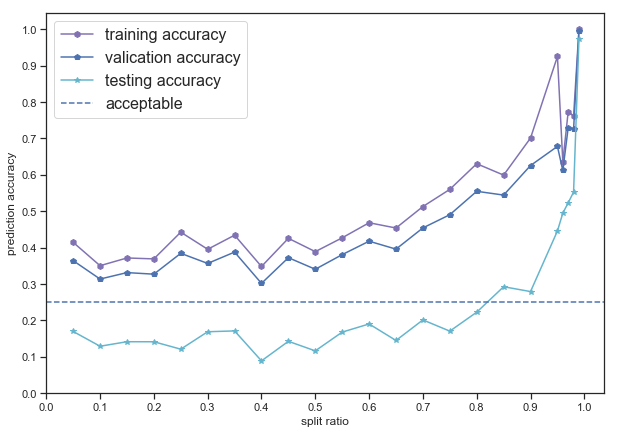
\includegraphics[width=0.7\textwidth]{figures/acc}
    \caption{Prediction accuracy with a limited context of input. This figure illustrates, with more context of clickstream
    known to the APM, more information to the model, and therefore much higher accuracy can be archived.
    The accuracy that evaluated here is a greedy search accuracy, and thus higher than 25\% of prediction accuracy is baseline,
    i.e., a quarter of future movements are predicted correctly.
    On the right side of the figure, the APM archived >60\% accuracy of 3 to 5 future steps prediction.
    Classification is a particular case in this figure where the split ratio is equal to 0.99.}
    \label{fig:acc}
\end{figure}

This figure illustrates, with more context of clickstream
feeds into the APM, the model receives more pieces of information of the clickstream.
Therefore much higher accuracy the APM can archive for prediction.
The accuracy of the APM evaluated here is \textbf{a greedy search accuracy}, which performs an element-wise comparison
between predicted clickstream and ground truth clickstream, and the accuracy is the number of
corrected predictions divided by the total number of prediction steps. 
Note that the greedy search is
used in this evaluation because the accuracy is compares ground truth and behaviors that APM learnt,
nevertheless, the beam search of APM that proposed in Section \ref{sec:optimization} is used for optimizing user
actions.

An accuracy that higher than 25\% is acceptable in the prediction task since it indicates
a quarter of future movements are predicted correctly.
On the right side of the figure, the APM archived >60\% accuracy of 3 to 5 future steps prediction.

Note that the prediction is still not overfitting to the dataset. Figure \ref{fig:loss}
illustrates the loss curve while training over 1500 epochs with three steps of prediction (split ratio 0.97).
The loss starts to increase after almost 200 epochs, which may be represented to overfitting.
Nevertheless, one can observe that the loss decreases down to a similar level of early training.
It archived a better performance (almost 60.0\% of precision) than previous, which indicates
the training process may re-parameterize the APM while training and archive better performance
for predictions.

\begin{figure}[H]
    \centering
    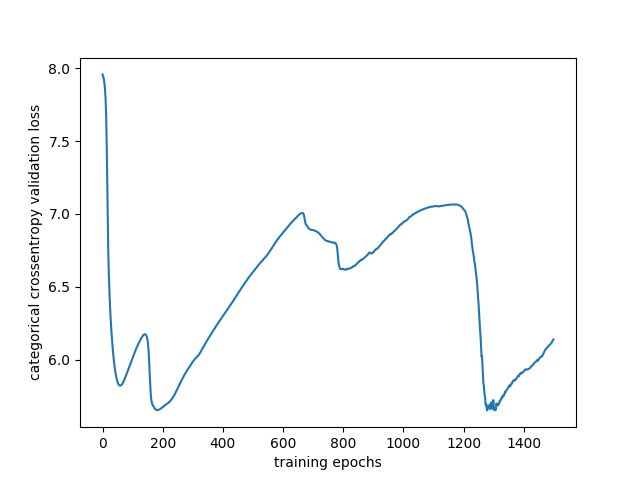
\includegraphics[width=0.55\textwidth]{figures/loss2}
    \caption{\emph{Validation loss} curve when the split ratio is 0.97. The loss indicates
    the model may be re-parameterized while training and archive better performance
    for predictions.}
    \label{fig:loss}
\end{figure}

\subsection{Action Path Visualization}

This section visualizes the actual action path of users and discusses the behavior qualitatively.
In total, 189 clickstreams are collected, which is not possible to illustrate all of them
in the thesis, the section selects the typical clickstreams to discuss and provides a visualization tool
(see Appendix \ref{appendix:a}) to help readers to explore all action paths.

\subsubsection{Individual Common Patterns}

\paragraph{Pattern of ``cluster''}
The first pattern one can observe from the goal-oriented task clickstream is called ``cluster''.
In Figure \ref{fig:vis-goal1} and \ref{fig:vis-goal2}, 
the visualization shows different clustered intents in Amazon's goal-oriented task. 
Formally, \emph{a pattern is called ``cluster'' if and only if it is a partition of an action path
that is connected with rest of the action path through a single node.}

\begin{figure}[H]
    \centering
    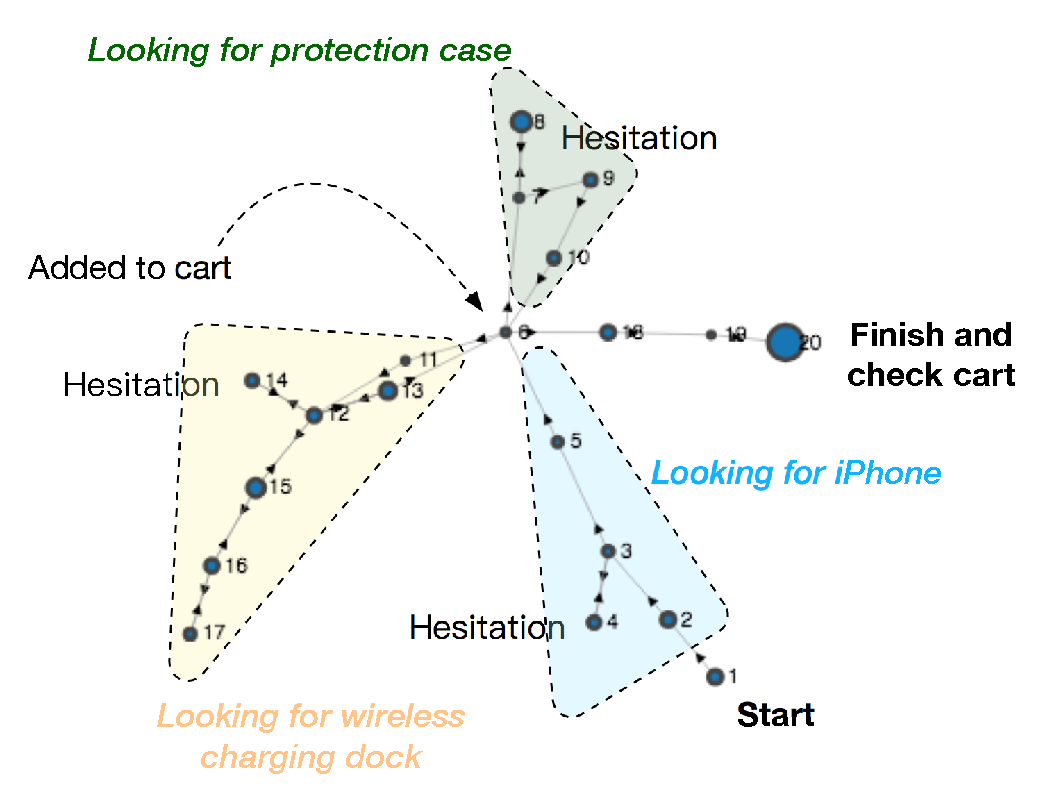
\includegraphics[width=0.55\textwidth]{figures/vis-goal1}
    \caption{Patterns of cluster and hesitation of an action path. This figure visualizes an action path in
    goal-oriented Amazon's task. The visualized graph can be partitioned into four subgraphs and three of them are cluster pattern that is a representing of different shopping intent, 
    which is exactly as same as the task design. Further, each cluster contains a hesitation pattern as labeled in the figure, for instance, the node labeled with 4, 8, 14 are hesitation. 
    Besides, the number of a node is a representative of a chronological serial number of user actions.}
    \label{fig:vis-goal1}
\end{figure}

One can easily discriminate the user browsing for 
different intent in a different cluster, and then finally went to the cart without
backtracking.

\paragraph{Pattern of ``hesitation''}
Beyond the cluster pattern, ``hesitation'' pattern is also observed in goal-oriented tasks
where a short child path branch from its parent node in each intent cluster, e.g. node
4, 8, 14 in Figure \ref{fig:vis-goal1} and node 5, 16 in Figure \ref{fig:vis-goal2},
which suggests ``hesitation'' is a pattern that more often appears in the goal-oriented task
within a ``cluster''. Formally, \emph{a pattern is called ``hesitation'' if and only if it
is an acyclic list and not in a star that joint with a cluster or a ring and the number of its nodes is less than any 
of the existed cluster.}

\paragraph{Pattern of ``ring'' and ``star''}
Similarly, in the fuzzy and exploring task, two common patterns ``ring'' and ``star''
patterns are observed that more often to appear in fuzzy and exploring tasks.
Formally, \emph{a pattern is called ``ring'' if and only if it is a list without connection to a cluster
and starting node is not joint with ending node; a pattern is called ``star'' if and only if 
it is a spanning tree of an action path that a non-leaf node contains more than one child.}


Figure \ref{fig:vis-fuzzy-explore1} illustrates an action path of Amazon's fuzzy task (purple nodes)
and an action path of Dribbble's exploring task (orange nodes), both from same participants.
One can observe ``ring'' and ``star'' patterns in the figure as highlighted through 
the gray area surrounded by a dashed line.


\begin{figure}[H]
    \centering
    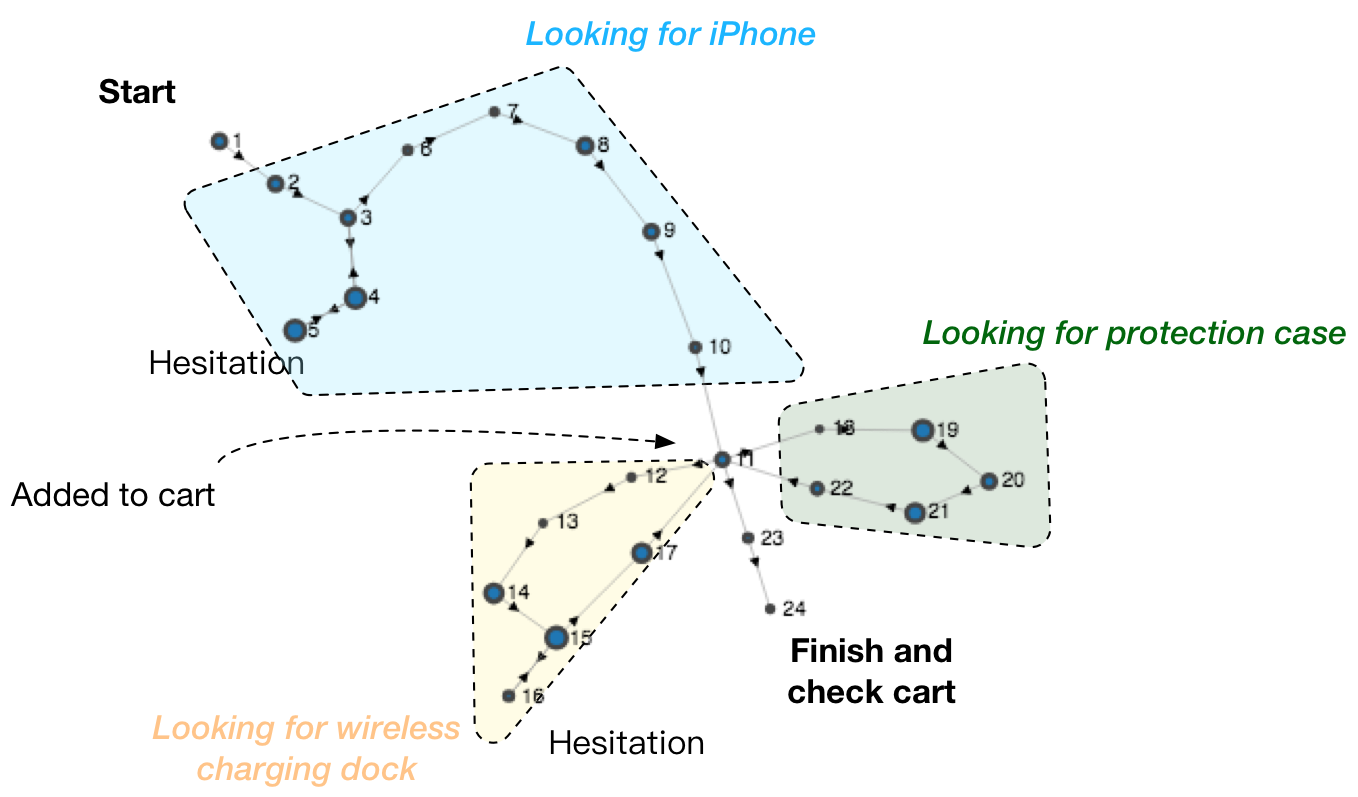
\includegraphics[width=0.55\textwidth]{figures/vis-goal2}
    \caption{Patterns of cluster and hesitation of an action path. This figure visualizes an action path in
    goal-oriented Amazon's task. The visualized graph can be partitioned into four subgraphs and three of them are cluster pattern that is a representing of different shopping intent, 
    which is exactly as same as the task design. Further, two of the clusters contain a hesitation pattern as labeled in the figure, for instance, the node labeled with 5, 16 is hesitation. 
    Besides, the number of a node
    is a representative of a chronological serial number of user actions.}
    \label{fig:vis-goal2}
\end{figure}

\begin{figure}[H]
    \centering
    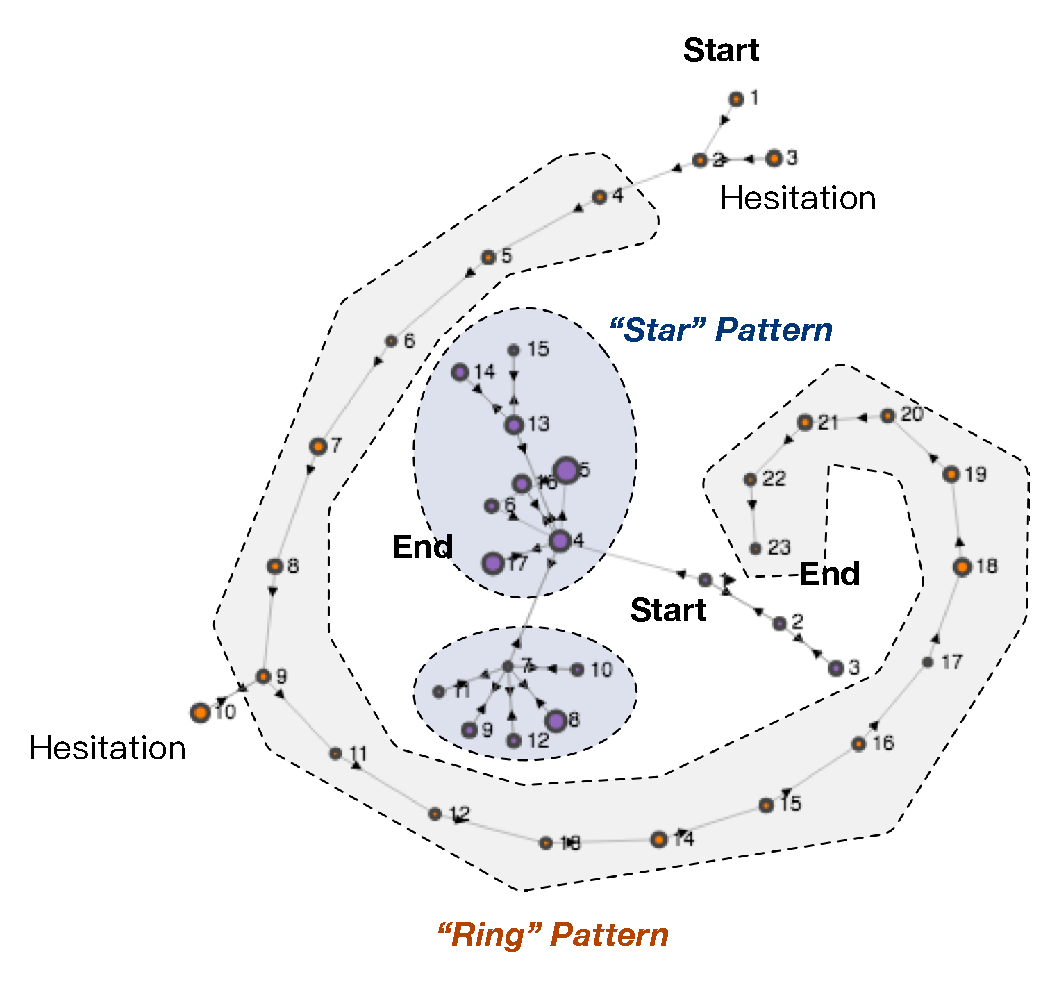
\includegraphics[width=0.55\textwidth]{figures/vis-patterns1}
    \caption{Patterns of ring and star of an action path. The figure visualizes an action path in
    Amazon's fuzzy browsing task (purple nodes) and Dribbble's exploring tasks (orange nodes). 
    The visualized action path of exploring task is a linked list with few hesitations (node 3 and 10).
    The action path of fuzzy task contains two star patterns (roots are 4 and 7).
    As same as other visualizations, the number of a node
    is a representative of a chronological serial number of user actions.}
    \label{fig:vis-fuzzy-explore1}
\end{figure}

Similarly, as one more illustration, Figure \ref{fig:vis-fuzzy-explore2} gives action paths 
in the same tasks but from another participant that the purple nodes represent actions in Amazon's fuzzy task action path
and orange nodes represent actions in Dribbble's exploring task action path.


In addition, even though the author observed that the number of star pattern is more often to appear
in fuzzy tasks and ring pattern is more often to appear in exploring tasks.
The author argues that this is because, in fuzzy tasks, participants can identify the
information uses, therefore the star pattern is more often to appear since it produces many backtracking
behavior and causes the ``differentiating'' activity. However, in the exploring task,
there is no explicit information uses described the exploring task, therefore participants
keep exploring deeper and deeper from the starting page without backtracking, the star pattern
appears when a participant has multiple interests on different pages that referred from the same page.

\begin{figure}[H]
    \centering
    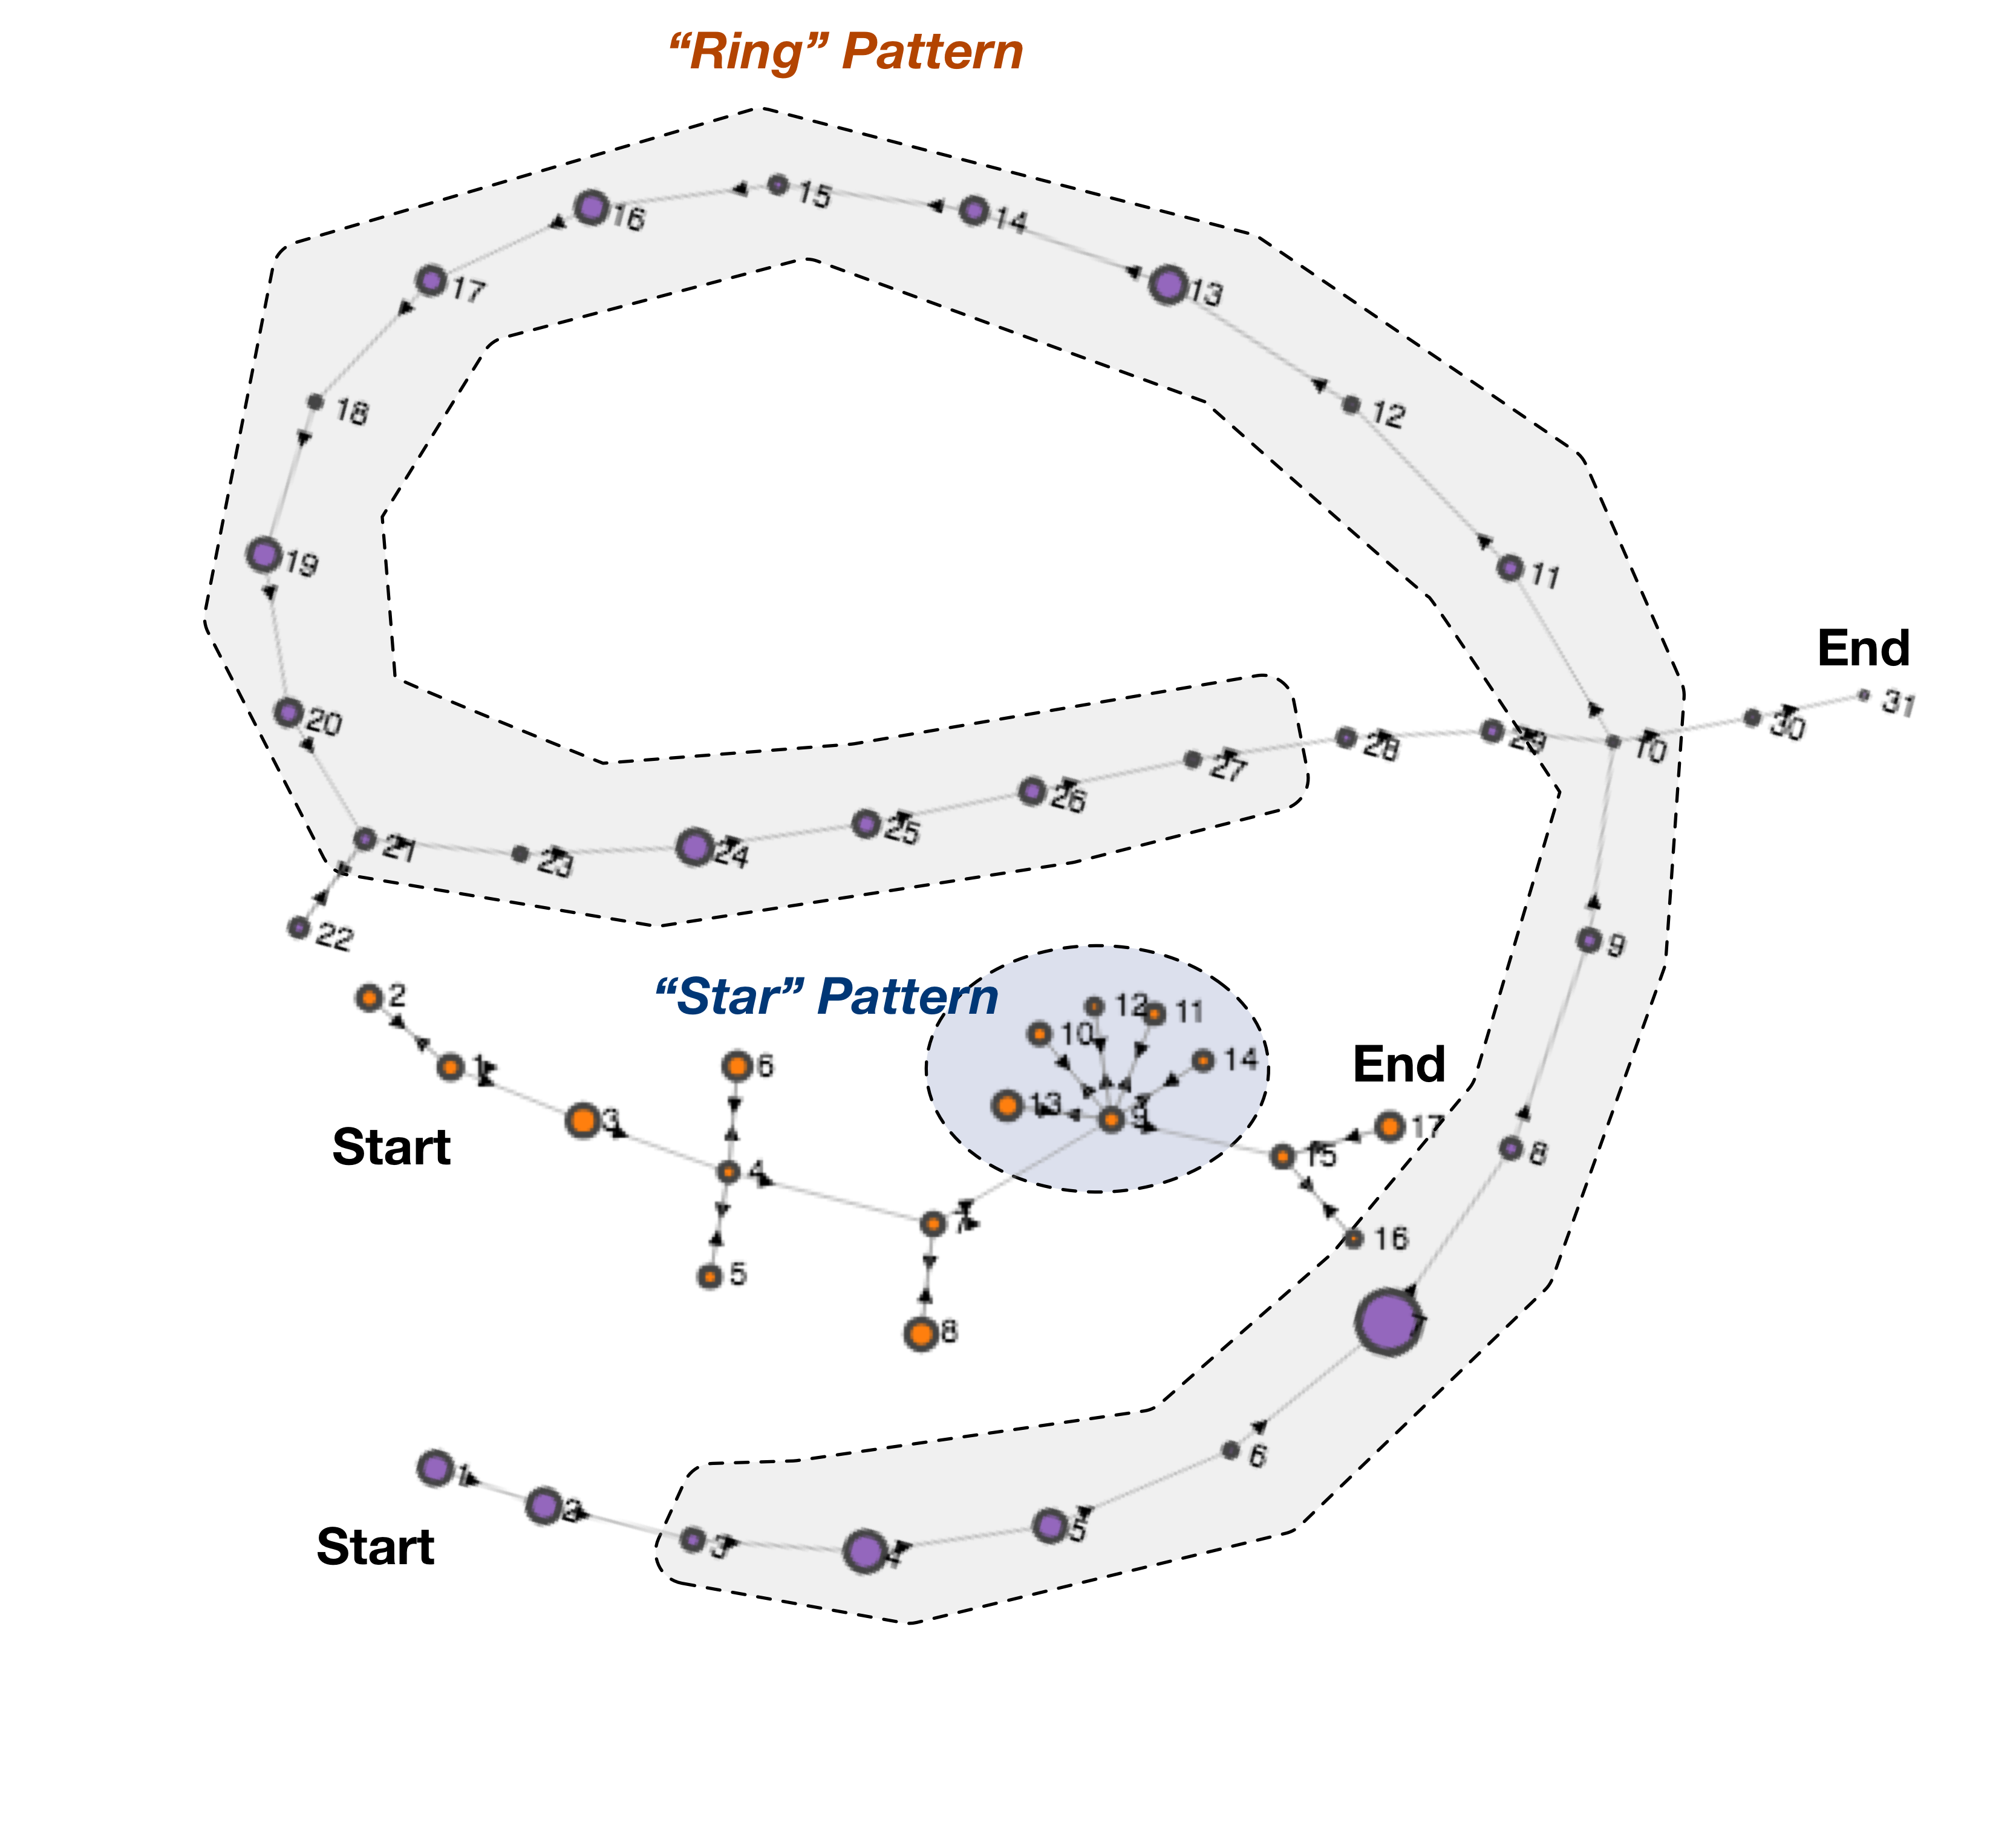
\includegraphics[width=0.55\textwidth]{figures/vis-patterns2}
    \caption{Patterns of ring and star of an action path. The figure visualizes an action path
    of a different participant in
    Amazon's fuzzy browsing task (purple nodes) and Dribbble's exploring tasks (orange nodes). 
    The visualized action path of exploring task contains a star pattern where the root is 9.
    The action path of fuzzy task contains a cyclic ring pattern that with a single hesitation
    in node 22.
    As same as other visualizations, the number of a node
    is a representative of a chronological serial number of user actions.}
    \label{fig:vis-fuzzy-explore2}
\end{figure}

In summary, one can conclude that:

\begin{enumerate}
    \item Goal-oriented browsing behavior contains common patterns of ``cluster'', and each cluster tend to indicate a specific intent;
    \item Fuzzy and exploring behavior two common pattern of ``ring'' and ``star'', however, ring pattern is more often to appear 
          in exploring behavior and star pattern is more often to appear in fuzzy behavior;
    \item Pattern of ``hesitation'' usually attached to a cluster or a ring but not appear in a star.
\end{enumerate}

\subsubsection{Cross user Overlap Patterns}

In the previous discussion, the common patterns are discussed that appears in individuals.
Nevertheless, it is still interesting to explore how action paths are manifest to multiple
participants. Fortunately, there are intersections among multiple subjects.

\paragraph{Pattern of ``overlap''}
occurs when observing action paths on multiple participants. Figure \ref{fig:overlap-example-1}
and \ref{fig:overlap-example-2} are the action paths visualized for \textbf{the same four participants}
in Medium's goal-oriented task, and Dribbble's exploring task respectively.
One can define a $n-$overlap ratio is the number of blackening nodes divided by the total number of nodes
in the action paths of $n$ participants. According to the definition, the maximum number of $4-$overlap ratio
is 100.00\%, and the minimum $4-$overlap ratio is 0.00\%.

However, the highest $4-$overlap ratio that observed from the
dataset is 11.84\% in the goal-oriented task. The lowest $4-$overlap ratio is 0.00\% 
when compare two different tasks.
Therefore, the author argue that the browsing behavior tends to be \emph{user-specific} 
even users have the same goal in a task. However, they still share similar overlaps 
which suggest \emph{common interests} between subjects.

In exploring task, the $4-$highest overlap ratio is 1.15\%, which is showed in Figure \ref{fig:overlap-example-2}.
The only common blacken node the starting page.
This observation suggests that exploring browsing behavior is highly user-specific.
Therefore, in conclusion, the overlap pattern of action path among multiple users suggests:

\begin{itemize}
    \item Browsing behavior tends to be user-specific. 
    However, it is unclear whether it is user-specific 
    because the APM have an issue with lack of data, which is discussed in Section \ref{sec:limitations}.
    \item Specifically, in goal-oriented browsing behavior, 
    one can observe common interests between multiple subjects,
    whereas the exploring tasks have no intersection between subjects.
\end{itemize}

\begin{figure}[H]
    \centering
    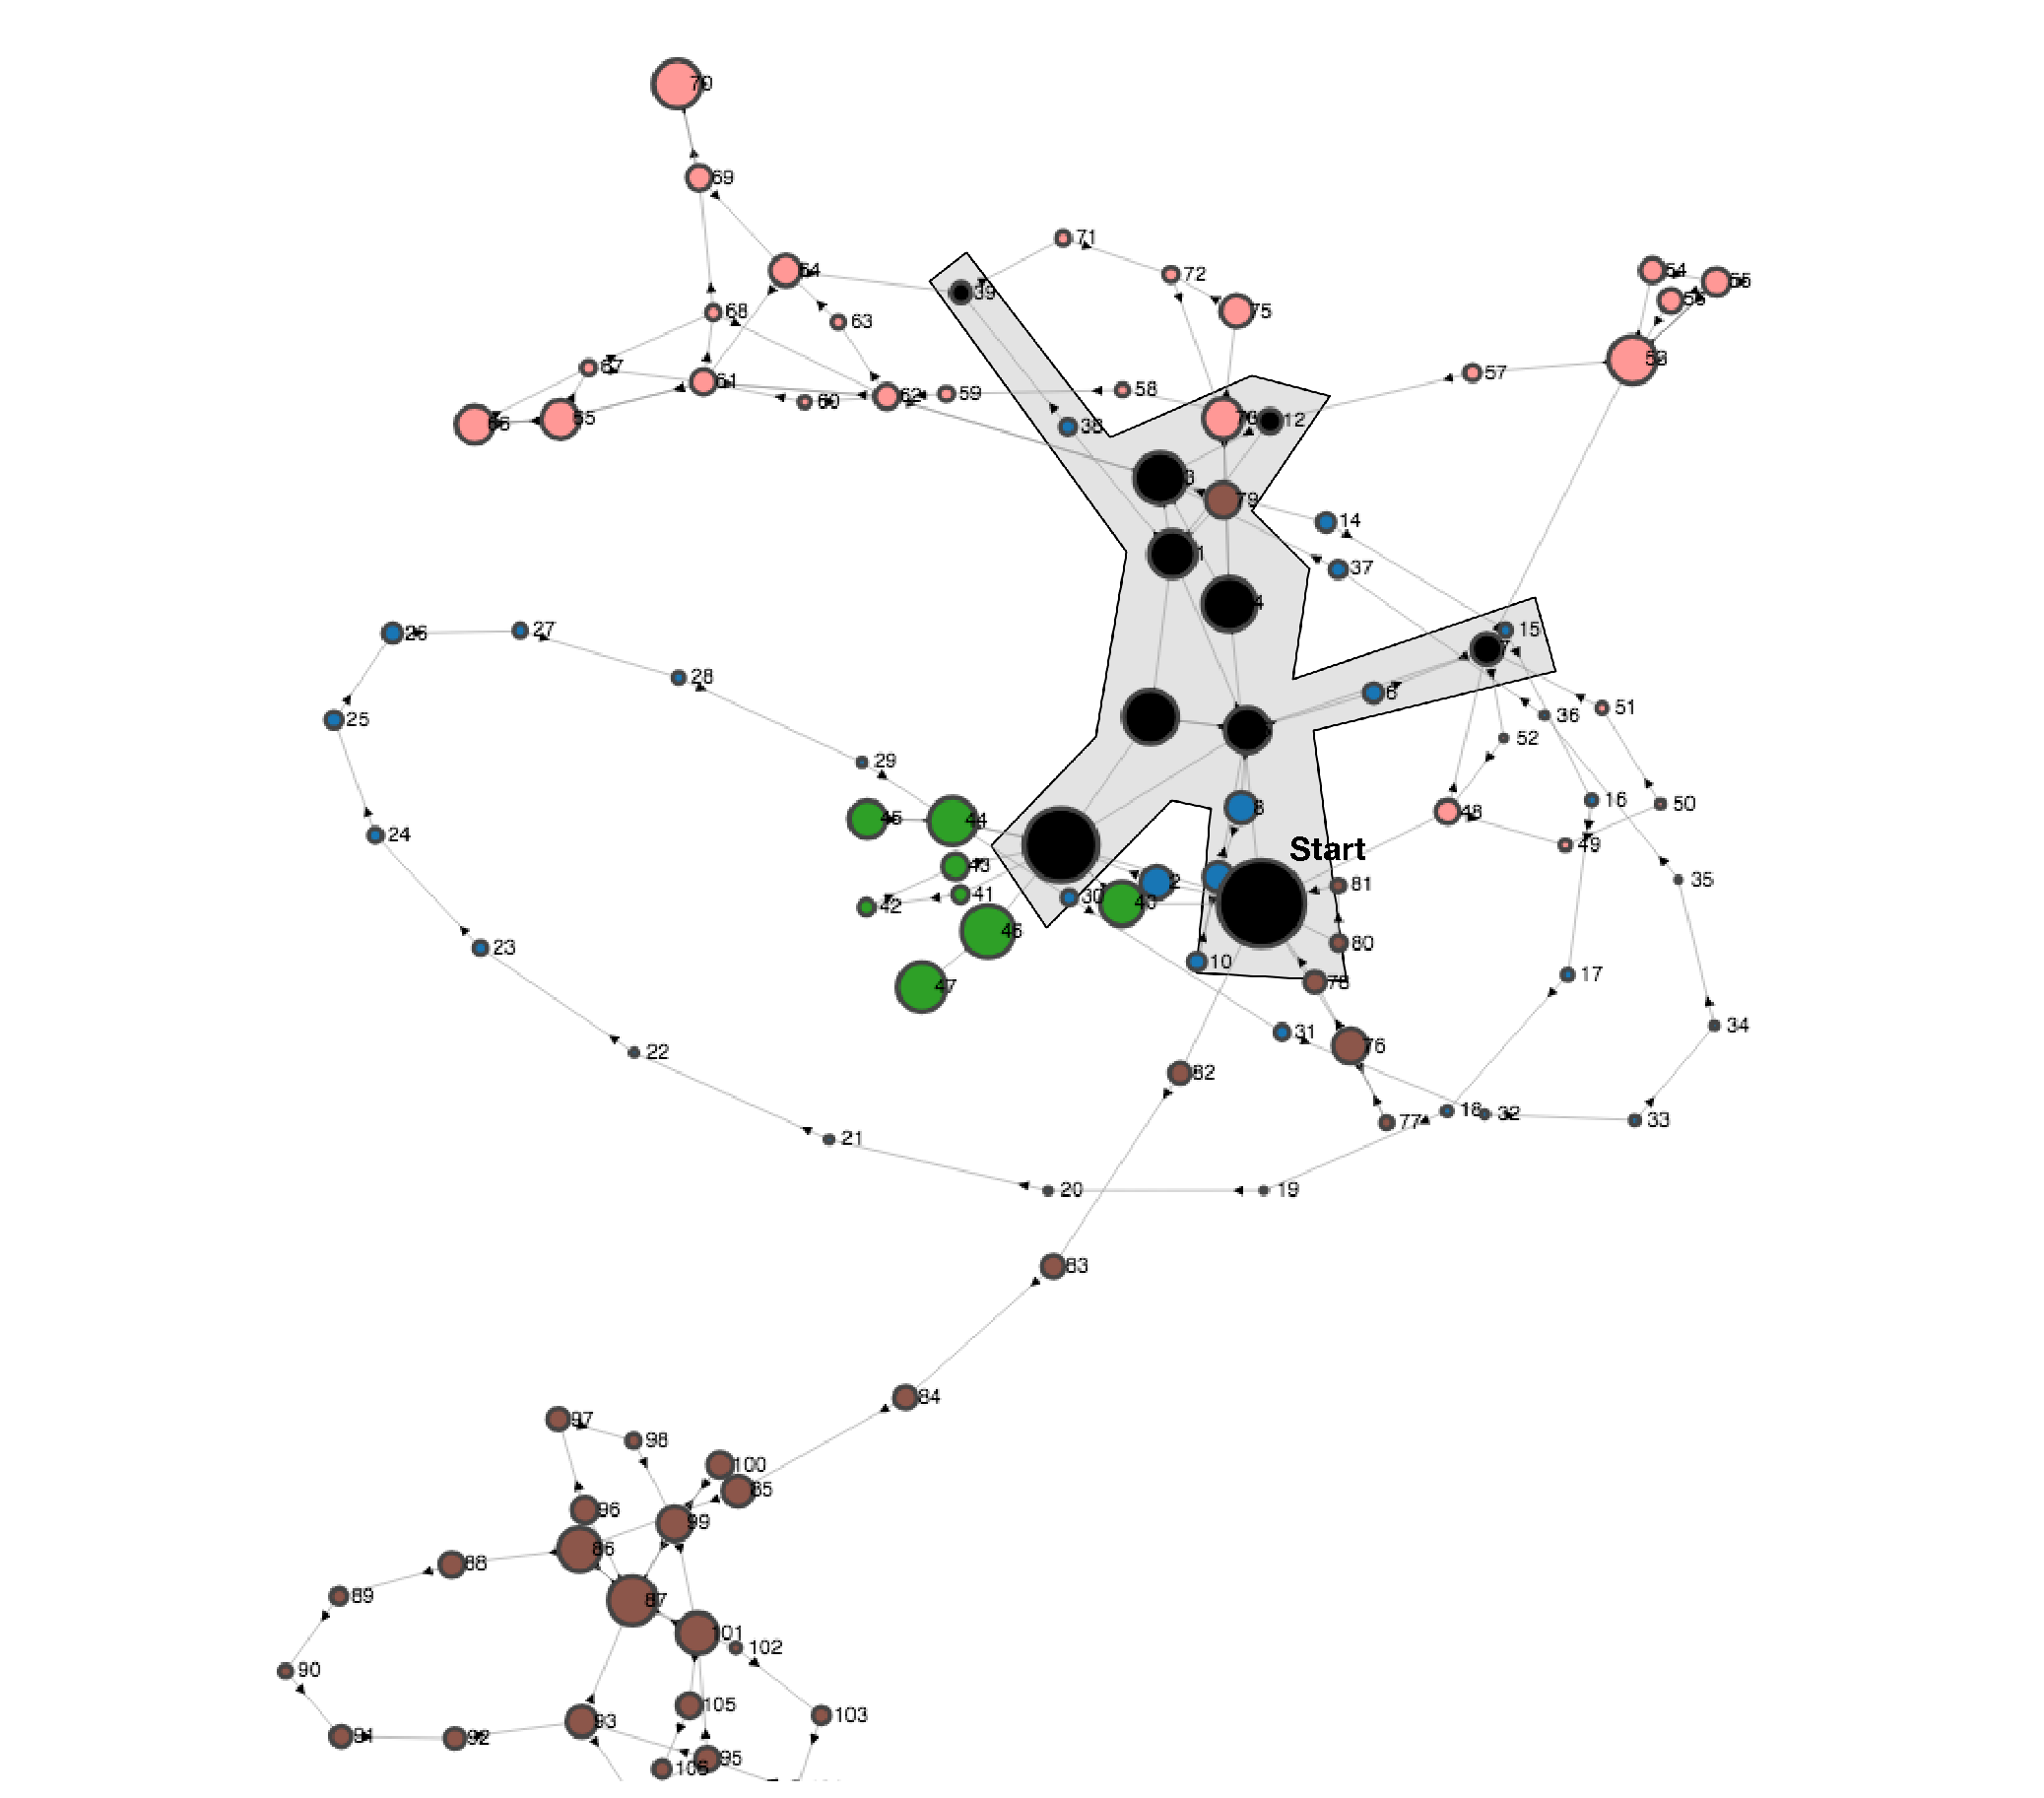
\includegraphics[width=1\textwidth]{figures/overlap1}
    \caption{Example of ``overlap'' pattern in Medium's goal-oriented task: 
    This figure visualizes the clickstream intersection 
    of four participants at Medium's goal-oriented task. 
    Each color represents an individual clickstream except black nodes, 
    which represents the overlapping of different clickstreams.
    The overlap ratio of this graph is 9.43\%.}
    \label{fig:overlap-example-1}
\end{figure}

\begin{figure}[H]
    \centering
    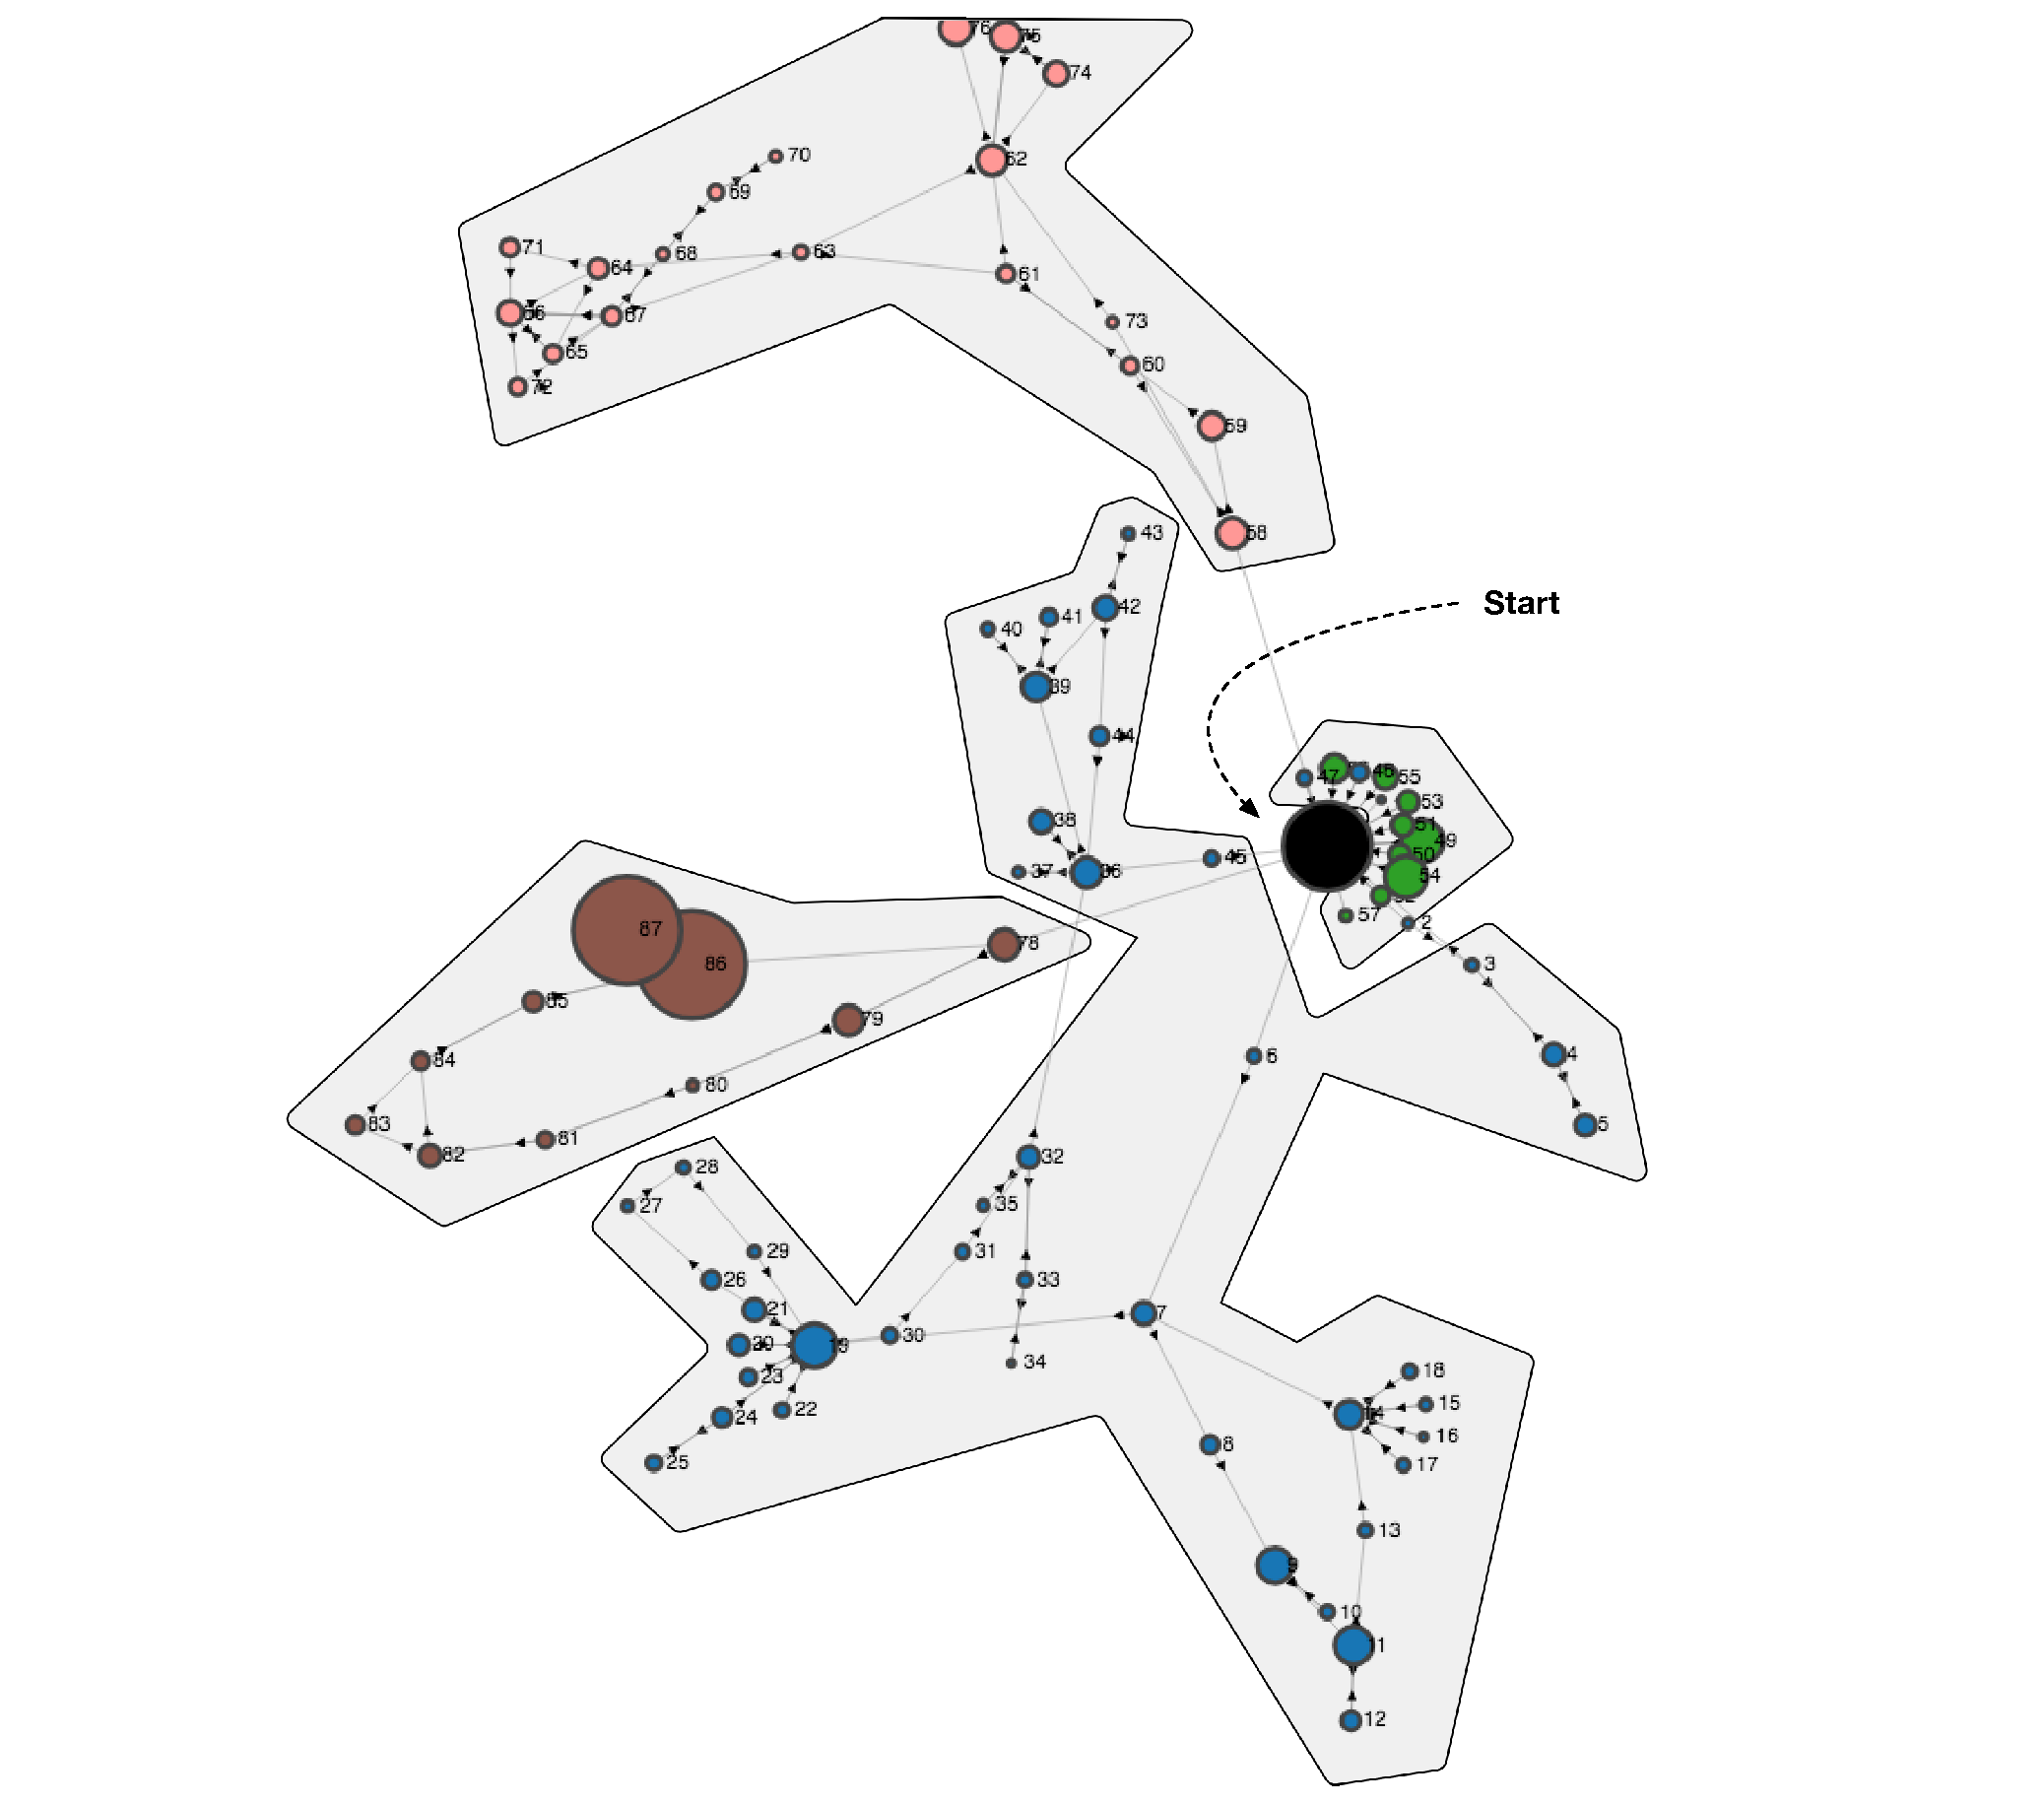
\includegraphics[width=1\textwidth]{figures/overlap2}
    \caption{Example of ``overlap'' pattern in Dribbble's exploring task: \
    This figure visualizes the clickstream intersection of four participants at Dribbble's exploring task. Each color represents an individual clickstream except blacken nodes, which represents the overlapping of different clickstreams.
    The overlap ratio of this graph is 1.15\%.}
    \label{fig:overlap-example-2}
\end{figure}

\paragraph{Remark} Table \ref{table:ellis-pattern} shows an analysis of all observed patterns
based on Ellis' model, which explains why these patterns exist and how they contribute to the APM.

\begin{table}[H]
    \small
    \centering
    \caption{Existence of activities from Ellis' Model and information use in the observed patterns
    The ``exist'', in the table, represents the existence of which activities contributes in which pattern.
    The ``observed'' indicates that the information need is observed from browsing behavior.}
    \begin{adjustbox}{width=\textwidth}
        \begin{tabular}{ccccccccc}
            \toprule
            \multicolumn{1}{c}{\multirow{2}{*}{\textbf{Behaviors}}}  & \multicolumn{1}{c}{\multirow{2}{*}{\textbf{Information Need}}} & \multicolumn{6}{c}{\textbf{Information Seeking}}                                    & \multicolumn{1}{c}{\multirow{2}{*}{\textbf{Information Use}}} \\ \cline{3-8}
            \multicolumn{1}{c}{}                                     & \multicolumn{1}{c}{}                                  & \textbf{Starting} & \textbf{Chaining} & \textbf{Browsing} & \textbf{Differentiating} & \textbf{Monitoring} & \textbf{Extracting} & \multicolumn{1}{c}{}  \\
            \hline
            cluster    &   observed &       &       &       & Exist & Exist & Exist & Exist \\
            star       &            &       & Exist & Exist & Exist &       &       &       \\
            ring       &            & Exist & Exist &       &       &       &       &       \\
            hesitation &   observed &       & Exist &       & Exist & Exist &       &       \\
            overlap    &   observed &       &       &       &       &       & Exist & Exist \\
            \bottomrule
        \end{tabular}
        \label{table:ellis-pattern}
    \end{adjustbox}
\end{table}

\begin{itemize}
    \item For ``cluster'' pattern, as discussed before, 
    information need can be observed from action path behavior,
    and the differentiating and monitoring contributes to the partitioning character 
    of the pattern and extracting and information then contributes to 
    the short ring and hesitations because the information is specified clearly.
    \item For ``star'' pattern, one can neither observe information need from action path 
    nor did the participant uses information that finds in the star pattern. 
    In Ellis' model, chaining, browsing and differentiating contributes to this pattern 
    since the depth from root to leaf node are small.
    \item For ``ring'' pattern, one can neither observe information need or information use. 
    The user explores deeper and deeper along the ring until the user exit the browsing session.
    \item For ``hesitation'', it connects to ring and cluster pattern, 
    therefore they have common activities of chaining, differentiating and monitoring.
    However, information from hesitations are not used, but one can easily observe the hesitation.
    \item For ``overlap'', one can observe common interests, which indicates information needs 
    and use, the extracting and information use contributes more to represent this behavior.
\end{itemize}

Combining with Table \ref{table:ellis}, ``cluster'' pattern and ``overlap'' pattern 
essentially contributes to goal-oriented browsing behavior since they share common activities 
in this behavior, 
``star'' and ``ring'' patterns contributes more on fuzzy and exploring tasks 
since their activities are more close to these browsing behaviors. 
Besides, as discussed before, these patterns cannot be observed with explicit information use.
The ``hesitation'' pattern appears in ``star'', ``ring'' and ``cluster'' pattern 
because they have common activities, such as ``chaining'' and ``differentiating''.

\cleardoublepage